% Data: completed presentation/BALANCED_INTERLEAVED_AMORTIZATION.csv.
% Filter: observed_native_edges, contract_exact, budgets 16*horizon,
% CG1 and budgeted_retest_all. Counts aggregate three recorded passes.
\begin{figure}[t]
\centering
\begingroup
\definecolor{resultblue}{HTML}{0072B2}
\definecolor{resultorange}{HTML}{D55E00}
\newcommand{\resultrequestpanel}[4]{%
  \foreach \tick in {0,64,128,192,256} {
    \draw[black!12] (0,\tick) -- (12,\tick);
    \node[anchor=east] at (-0.35,\tick) {\tick};
  }
  \draw[black!65] (0,0) -- (12,0);
  \draw[black!65] (0,0) -- (0,290);
  \draw[resultorange,thick,densely dashed] (0,64) -- (4,128) -- (12,256);
  \foreach \x/\y in {0/64,4/128,12/256}
    \node[rectangle,draw=resultorange,fill=white,minimum size=5pt,
      inner sep=0pt] at (\x,\y) {};
  \draw[resultblue,thick] (0,#2) -- (4,#3) -- (12,#4);
  \foreach \x/\y in {0/#2,4/#3,12/#4}
    \fill[resultblue] (\x,\y) circle[radius=1.9pt];
  \node[anchor=west,fill=white,inner sep=1pt] at (0,86) {#2/64};
  \node[fill=white,inner sep=1pt] at (4,150) {#3/128};
  \node[anchor=east,fill=white,inner sep=1pt] at (12,278) {#4/256};
  \foreach \x/\label in {0/4,4/8,12/16}
    \node[below] at (\x,-7) {\label};
  \node at (6,322) {\textbf{#1: requests}};
}
\newcommand{\resultdetectionpanel}[3]{%
  \foreach \tick/\label in {0/0,0.5/0.5,1/1} {
    \draw[black!12] (0,\tick) -- (12,\tick);
    \node[anchor=east] at (-0.35,\tick) {\label};
  }
  \draw[black!65] (0,0) -- (12,0);
  \draw[black!65] (0,0) -- (0,1.05);
  \draw[resultorange,thick,densely dashed] (0,1) -- (4,1) -- (12,1);
  \foreach \x in {0,4,12}
    \node[rectangle,draw=resultorange,fill=white,minimum size=5pt,
      inner sep=0pt] at (\x,1) {};
  \draw[resultblue,thick] (0,0.5) -- (4,#2) -- (12,1);
  \foreach \x/\y in {0/0.5,4/#2,12/1}
    \fill[resultblue] (\x,\y) circle[radius=1.9pt];
  \node[anchor=west,fill=white,inner sep=1pt] at (0,1.13) {12/12};
  \node[fill=white,inner sep=1pt] at (4,1.13) {24/24};
  \node[anchor=east,fill=white,inner sep=1pt] at (12,1.13) {48/48};
  \node[anchor=west,fill=white,inner sep=1pt] at (0,0.36) {6/12};
  \node[fill=white,inner sep=1pt] at (4,{#2-0.14}) {#3/24};
  \node[anchor=east,fill=white,inner sep=1pt] at (12,0.86) {48/48};
  \foreach \x/\label in {0/4,4/8,12/16}
    \node[below] at (\x,-0.04) {\label};
  \node at (6,-0.29) {Changes};
  \node at (6,1.42) {\textbf{#1: detection fraction}};
}
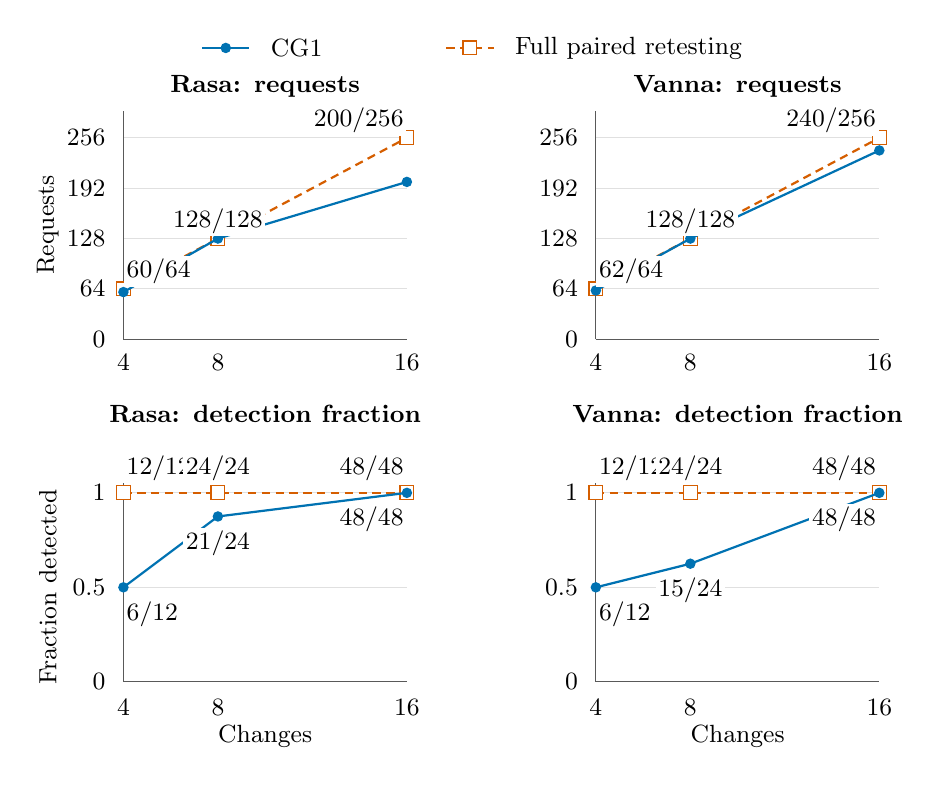
\begin{tikzpicture}[font=\small]
  \draw[resultblue,thick] (1.0,8.05) -- (1.6,8.05);
  \fill[resultblue] (1.3,8.05) circle[radius=1.9pt];
  \node[anchor=west] at (1.75,8.05) {CG1};
  \draw[resultorange,thick,densely dashed] (4.1,8.05) -- (4.7,8.05);
  \node[rectangle,draw=resultorange,fill=white,minimum size=5pt,
    inner sep=0pt] at (4.4,8.05) {};
  \node[anchor=west] at (4.85,8.05) {Full paired retesting};
  \begin{scope}[x=0.30cm,y=0.010cm,yshift=4.35cm]
    \resultrequestpanel{Rasa}{60}{128}{200}
    \node[rotate=90] at (-3.2,145) {Requests};
  \end{scope}
  \begin{scope}[x=0.30cm,y=0.010cm,xshift=6.0cm,yshift=4.35cm]
    \resultrequestpanel{Vanna}{62}{128}{240}
  \end{scope}
  \begin{scope}[x=0.30cm,y=2.4cm]
    \resultdetectionpanel{Rasa}{0.875}{21}
    \node[rotate=90] at (-3.2,0.5) {Fraction detected};
  \end{scope}
  \begin{scope}[x=0.30cm,y=2.4cm,xshift=6.0cm]
    \resultdetectionpanel{Vanna}{0.625}{15}
  \end{scope}
\end{tikzpicture}
\endgroup
\caption{Exact-state reuse in the balanced interleaved replay, with observed
edges and exact judgments. Native task-request labels are CG1/full retesting per trajectory;
ceilings are 64, 128 and 256 for 4, 8 and 16 changes. Detection labels are
detected/repeated reference opportunities across three recorded passes. Keeping
cost and detection separate exposes early missed opportunities: smaller request
counts at four changes do not preserve full detection. At sixteen changes,
CG1 matches full detection with 200 versus 256 requests in Rasa and 240 versus
256 in Vanna. These savings depend on revisiting identical H/A/B states and
are shared by other selective arms. Connecting lines guide the eye between
the three evaluated horizons.}
\Description{Four line panels separate request costs and detection fractions.
At 4, 8 and 16 changes, Rasa CG1 uses 60, 128 and 200 requests, while Vanna
CG1 uses 62, 128 and 240; full retesting uses 64, 128 and 256 in both settings.
Rasa CG1 detects 6 of 12, 21 of 24 and 48 of 48 repeated opportunities; Vanna
CG1 detects 6 of 12, 15 of 24 and 48 of 48. Full retesting detects 12 of 12,
24 of 24 and 48 of 48 in both settings. Exact-state recurrence permits profile
reuse. All fractions aggregate three recorded passes.}
\label{fig:result-reuse}
\end{figure}
